\documentclass[12pt, a4paper]{report}
\setcounter{secnumdepth}{0}
\usepackage{graphicx}
\usepackage{titlesec}
\usepackage{pdfpages}
\usepackage{wrapfig}
\usepackage{dirtree}
\usepackage{listings}
\usepackage{xcolor}
\usepackage{hyperref}
\usepackage[T1]{fontenc}
\usepackage[utf8]{inputenc}

\graphicspath{ {./images/} }

\definecolor{light-gray}{gray}{0.95}
\definecolor{codeviolet}{rgb}{0.478, 0.321, 0.639}
\definecolor{codegreen}{rgb}{0.266, 0.549, 0.152}
\definecolor{backcolor}{rgb}{0.968, 0.952, 0.835}
\definecolor{codegray}{rgb}{0.466, 0.466, 0.466}
\definecolor{codeblue}{rgb}{0.294, 0.411, 0.776}
\newcommand{\code}[1]{\colorbox{light-gray}{\texttt{#1}}}

% defining code block style
\lstdefinestyle{mystyle}{
    backgroundcolor=\color{backcolor},   
    commentstyle=\color{codegreen},
    keywordstyle=\color{codeblue},
    numberstyle=\tiny\color{codegray},
    stringstyle=\color{codegray},
    basicstyle=\ttfamily\footnotesize,
    breakatwhitespace=false,         
    breaklines=true,                 
    captionpos=b,                    
    keepspaces=true,                 
    numbers=left,                    
    numbersep=5pt,                  
    showspaces=false,                
    showstringspaces=false,
    showtabs=false,                  
    tabsize=4
}
\lstset{style=mystyle}

\title{
  \begin{huge}
    \textbf{
      {Computer Science Project 2020-'21}\\
      {Sudoku Web App}
    }\\
  \end{huge}
  \begin{figure}
      \centering
      {
\includegraphics[scale=2]{iss}}
  \end{figure}
}
\author{
x % add only one name here
}

\date{\vspace{-5ex}}

\begin{document}

  \begin{titlepage}
  \maketitle
  \end{titlepage}

  \newpage
  
\includepdf{cert}
  
  \newpage
  \maketitle
  \begin{large}
  \section*{Acknowledgements}
  I have taken efforts in this project. However, it would not have been possible without the kind support and help of many individuals and organizations. I would like to extend my sincere thanks to all of them. \newline
  \newline
  I am greatly indebted to the teacher-in-charge, Ms.~Deepa Dinesh for her guidance and constant supervision as well as for providing necessary information 
  regarding the project and also for her support in completing the project. \newline
  \newline
  I would like to express my gratitude towards my parents for their kind cooperation and encouragement which helped me in the completion of this project. \newline
  \newline
  I would also like to express my special gratitude and thanks to my classmates in developing the project and to the people who have willingly 
  helped me out with their abilities.
  \end{large}
  
  
  \maketitle    % table of contents page
  \begin{large}
  \newpage
  \tableofcontents
  \end{large}
  
  
  \newpage
  \section{Introduction}
  Python was created in the late 1980s, and first released in 1991, by Guido van Rossum as a successor to the ABC programming language.
  \begin{wrapfigure}{r}{0.25\textwidth}
    
\includegraphics[width=0.25\textwidth]{introduction}
  \end{wrapfigure}
  Python is an interpreted, object-oriented, high-level programming language with dynamic semantics. Its high-level built in data structures, combined with dynamic typing and dynamic binding, make it very attractive for Rapid Application Development, as well as for use as a scripting or glue language to connect existing components together.

  Python's simple, easy to learn syntax emphasizes readability and therefore reduces the cost of program maintenance. Python supports modules and packages, which encourages program modularity and code reuse. The Python interpreter and the extensive standard library are available in source or binary form without charge for all major platforms, and can be freely distributed.
  
  \subsection{Features in Python:}
    \subsubsection{Easy to code:}
    Python is a high-level programming language. Python is very easy to learn as compared to other languages like C, C#, JavaScript, Java, etc. It is very easy to code in python language and anybody can learn python basics in a few hours or days. It is also a developer-friendly language.
    
    \subsubsection{Free and Open Source:}
    Since it is open-source, this means that source code is also available to the public. So you can download it as, use it as well as share it.
    
    \subsubsection{Object-Oriented Language:}
    One of the key features of Python is Object-Oriented Programming. Python supports object-oriented language and concepts of classes, objects, encapsulation, etc.
    
    \subsubsection{High-Level Language:}
    Python is a high-level language. When we write programs in Python, we do not need to remember the system architecture or manage memory.
    
  \newpage
  \section{Feasibility Study}
   The feasibility study is the important step in any software development process. This is because it makes analysis of different aspects like - cost required for developing and executing the system, the time required for each phase of the system and so on. If these important factors are not analyzed then definitely it would have impact on the organization & the development and the system would be a total failure.

  The purpose of feasibility study is not to solve the problem, but to determine whether the problem is worth solving. By making analysis this way it would be possible to make a report of identified area of problem. By making a detailed analysis in this area a detailed document or report is prepared in this phase which has details like project plan or schedule of the project, the cost estimated for developing and executing the system, target dates for each phase of delivery of system developed and so on. This phase is the base of software development process since further steps taken in software development life cycle would be based on the analysis made on this phase and so careful analysis has to be made in this phase.
  
  \subsection{TELOS}
  
    The feasibility study concentrates on the following area (TELOS):
    \begin{itemize}
      \item Technology and System Feasibility
      \item Economic Feasibility
      \item Legal Feasibility
      \item Operational Feasibility
      \item Schedule Feasibility
    \end{itemize}
  
    \subsubsection{Technology and System Feasibility}
    The assessment is based on an outline design of system requirements, to determine whether the company has the technical expertise to handle completion of the project.
  
    \subsubsection{Economic Feasibility}
    The economic feasibility study evaluates the cost of the software development against the ultimate income or benefits expected from the developed system. It includes identifying cost and benefit factors like - Development costs and Operating costs. There must be scopes for profit after the successful completion of the project.
  
    \subsubsection{Legal Feasibility}
    It determines whether the proposed system conflicts with legal requirements, e.g. a data processing system must comply with the local Data Protection Acts.
  
    \subsubsection{Operational Feasibility}
    Operational feasibility is a measure of how well a proposed system solves the problems, and takes advantage of the opportunities identified during scope definition and how it satisfies the requirements identified in the requirements analysis phase of system development.
  
    \subsubsection{Schedule Feasibility}
    A project will fail if it takes too long to be completed before it is useful. Typically this means estimating how long the system will take to develop, and if it can be completed in a given time period using some methods like payback period. Schedule feasibility is a measure of how reasonable the project timetable is. Given our technical expertise, are the project deadlines reasonable?
    
  \subsection{Advantages of Feasibility Study}
    \begin{itemize}
      \item As the initial step of software development life cycle, feasibility study has all the analysis part in it, which helps in analyzing the system requirements completely. 
      \item Helps in identifying the risk factors involved in developing and deploying the system.
      \item It helps in making cost/benefit analysis which helps the organization and system to run efficiently.
      \item It is a report which could be used by the senior or top persons in the organization. This is because, based on the report the organization decides about cost estimation, funding and other important decisions which is very essential for an organization to run profitably and for the system to run stable.
    \end{itemize}
    
  \subsection{Software Development Life Cycle}
  The Systems Development Life Cycle (SDLC) is a conceptual model used in project management that describes the stages involved in an information system development project from an initial feasibility study through maintenance of the completed application. \newline
  \begin{wrapfigure}{r}{0.25\textwidth}
    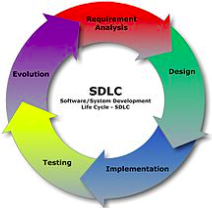
\includegraphics[width=0.25\textwidth]{feasibility-study}
  \end{wrapfigure}
  The following are the activities of the SDLC:
  \begin{itemize}
      \item Software requirement analysis
      \item Systems analysis and design
      \item Design/Code generation
      \item Testing
      \item Development and Maintenance
  \end{itemize}
  A Systems Development Life Cycle (SDLC) adheres to important phases that are essential for developers, such as planning, analysis, design, and implementation. A number of system development life cycle (SDLC) models have been created such as waterfall, fountain, spiral etc.
  
  \subsubsection{Requirement Analysis/Investigation}
  The 1st stage of SDLC is the investigation phase. During this stage, business opportunities and problems are identified, and information technology solutions are discussed. Multiple alternative projects may be suggested and their feasibility analyzed. The results of the feasibility study can then be compiled into a report, along with preliminary specifications. When the investigation stage ends, a decision whether or not to move forward with the project should be made.
  
  \subsubsection{System Analysis}
  The goal of system analysis is to determine where the problem is, in an attempt to fix the system. It analyzes the requirement for the proposed system. To understand the nature of the program to build, the system engineer must understand the information domain for the software, as well as required functions, performance and the interfacing. This step involves breaking down the system in different pieces to analyze the situation, analyzing project goals, breaking down what needs to be created. From the available information the system engineer develops a list of system level requirement for the project.
  
  \subsubsection{Design}
  Systems design describes screen layouts, business rules, process diagrams, a complete entity- relationship diagram with a full data dictionary and other documentation. It defines specifically how the software is to be written including an object model, the client/server technology, a detailed database design etc. These design elements are intended to describe the software in sufficient detail that skilled programmers may develop the software with minimal additional input design. Analysis and design are very important in the whole development cycle. Any glitch in the design could be very expensive to solve in the later stage of the software development. The design must be translated into a machine readable form.
  
  \subsubsection{Testing}
  In this stage, all the pieces of software are brought together into a special testing environment and then are checked for errors, bugs and interoperability. Unit, system and user acceptance testing is often performed.
  
  \subsubsection{Deployment and Maintenance}
  Deployment is the final stage of initial development. It involves installation, initial training and may involve hardware and network upgrades. Software will definitely undergo change once it is delivered to the customer. There may be many reasons for the change. Change could be due to some unexpected input values into the system. The software should be developed to accommodate changes that could take place during the post implementation period. Maintaining the system is also an important aspect of SDLC.
  
  
  \newpage
  \section{Hardware and Software}
    \subsection{Hardware}
    Lenovo Ideapad \newline
    \emph{Intel Core i5, 4GB RAM}
    
    \subsection{Software}
    \begin{enumerate}
        \item \textbf{Git SCM} \newline
        Git is a distributed version-control system for tracking changes in any set of files, originally designed for coordinating work among programmers cooperating on source code during software development. Its goals include speed, data integrity, and support for distributed, non-linear workflows (thousands of parallel branches running on different systems).
        \item \textbf{GitHub} \newline
        GitHub is a provider of Internet hosting for software development and version control using Git. It offers the distributed version control and source code management (SCM) functionality of Git, plus its own features. It provides access control and several collaboration features such as bug tracking, feature requests, task management, continuous integration and wikis for every project.
        \item \textbf{Google Cloud Platform} \newline
        Google Cloud Platform (GCP), offered by Google, is a suite of cloud computing services that runs on the same infrastructure that Google uses internally for its end-user products, such as Google Search, Gmail, file storage, and YouTube.
        \item \textbf{Gunicorn} \newline
        "Green Unicorn" is a Python Web Server Gateway Interface (WSGI) HTTP server. It is a pre-fork worker model, ported from Ruby's Unicorn project. The Gunicorn server is broadly compatible with a number of web frameworks, simply implemented, light on server resources and fairly fast.
        \item \textbf{Visual Studio Code} \newline
        It is a free source-code editor made by Microsoft for Windows, Linux and macOS. Features include support for debugging, syntax highlighting, intelligent code completion, snippets, code refactoring, and embedded Git.
        \item \textbf{PyCharm Community Edition} \newline
        PyCharm is an integrated development environment (IDE) used in computer programming, specifically for the Python language. It is developed by the Czech company JetBrains.
        \item \textbf{\LaTeX} \newline
        This project report was made using \LaTeX. \LaTeX is a high-quality typesetting system; it includes features designed for the production of technical and scientific documentation. \LaTeX is the de facto standard for the communication and publication of scientific documents.
        \item \textbf{Adobe Photoshop} \newline
        Adobe Photoshop is a raster graphics editor developed and published by Adobe Inc. for Windows and macOS.
    \end{enumerate}
    
    
  \newpage
  \section{About the Project}
  The aim of the project, Sudoku Webapp, is to provide an aesthetically rich interface for sudoku enthusiasts to enjoy sudoku puzzles.\newline

  A website with 3 webpages: home page, sudoku page and leaderboard page, is the frontend of the project with which the user interacts. The webpages are made using Django, HTML, JavaScript and a CSS framework called Tailwind. A MySQL database is the primary data store, and is used to store the leaderboard data, and the sudoku game boards that are served on the site.\newline

  A personal aim with this project was to see how much we, as a team, could push ourselves to make a good, functional service. It challenged our creativity, programming skills and our ability to work and co-operate as a team. This project was a great learning experience.

  
  \newpage
  \section{Source Code}
    \subsection{File Structure and Dependencies}
    \subsubsection{File Structure}
    A rough structure of the project is as follows:
    \dirtree{%
    .1 SudokuWebapp.
    .2 latex-report.
    .2 sudoku-django-project.
    .3 mainapp.
    .4 migrations.
    .4 static.
    .4 templates.
    .3 static.
    .3 sudoku.
    .3 utils.
    .3 manage.py.
    .3 requirements.txt.
    .2 .gitignore.
    .2 README.md.
    }
    \vspace{0.5cm}
    The \verb|SudokuWebapp| directory is the root of the repository, and contains the entire project.\\ Inside this, the \verb|sudoku-django-project| is the root of the \emph{Django project}, and is where all the code is held, while the \verb|latex-report| directory contains all the images and \LaTeX code used to make this report.\\
    The \verb|.gitignore| is a special file used by the Git SCM. All files that are meant to be ignored by the version-control system (and not committed to history) are included in this. \\
    The \verb|sudoku-django-project/requirements.txt| is where all project dependencies are listed.\\
    The entire source code of the project is hosted on our Github repository, and can be viewed at \url{https://www.github.com/cs-gang/sudokuwebapp}.
    
    \subsubsection{Dependencies}
    \texttt{%
    asgiref==3.2.10 \\
    cffi==1.14.3 \\
    cryptography==3.2.1 \\
    Django==3.1.2 \\
    django-mysql==3.9.0 \\
    flake8==3.8.4 \\
    gunicorn==20.0.4 \\
    mccabe==0.6.1 \\
    mysqlclient==2.0.1 \\
    protobuf==3.13.0 \\
    pycodestyle==2.6.0 \\
    pycparser==2.20 \\
    pyflakes==2.2.0 \\
    PyMySQL==0.10.1 \\
    pytz==2020.1 \\
    six==1.15.0 \\
    sqlparse==0.3.1 \\
    }
    \\
    \begin{footnotesize}
    All dependencies were installed in an isolated \emph{Virtual Environment}.\\
    This \verb|requirements.txt| file was auto-generated by using the \code{pip freeze > requirements.txt} command. 
    \end{footnotesize}
    
    \subsection{Backend}
    Backend, also referred to as the \emph{"server-side"}, is responsible for facilitating communication between the presentation layer and the data layer.\\
    The backend of this project is handled by the \emph{Django} web framework.\\
    \subsubsection{Django Project Architecture}
    Django uses two important terms in development: \emph{project} and \emph{app}.\\
    A \textbf{project} refers to the entire web application.\\
    An \textbf{app} refers to a sub-module, catering to one specific part of the project.\\
    In our case, the \emph{project} is \texttt{sudoku-django-project}. This project contains only one \emph{app}, called \texttt{mainapp}.\\
    Django, being a web framework, auto-generates a lot of files for us when we create a new project. Almost all the code in the \texttt{sudoku-django-project/sudoku} directory was made like this. They contain instructions and settings for the entire project itself.\\
    Some of these files are listed below:
    \begin{itemize}
        \item \textit{manage.py}\\
        Used to manage the project and run adminsitrative commands like running the built-in server.
        \item \textit{sudoku/settings.py}\\
        Contains most of the configuration for the Django project, like what databases to use, where to look for static files etc.
        \item \textit{sudoku/urls.py}\\
        Contains information about locations where URLs of the project has been declared.
    \end{itemize}
    The application folder \texttt{sudoku-django-project/mainapp} also contains many pre-made files.\\
    \\
    Django projects separates data (\emph{models}), the logic (\emph{view}) and the final presentation (\emph{template}) that users will see. This kind of architecture is hence called \textbf{MTV (Model Template View)} architecture.\\
    \begin{enumerate}
        \item A \textbf{model} is responsible for data management, and deals with access and relationships between data. Django uses an \textbf{ORM (Object Relational Mapping)} to make this process more intuitive.
        \item A \textbf{template} is responsible for presentation of data to the user. These are the HTML pages.
        \item A \textbf{view} acts like a bridge between models and templates. A view accesses model data and redirects it to a template for presentation.
    \end{enumerate}
    \textbf{Models}
    \begin{figure}[h!]
        \centering
        \includegraphics{game-board}
        \caption{Game boards table}
        \label{fig:game-boards}
    \end{figure}
    \begin{figure}[h!]
        \centering
        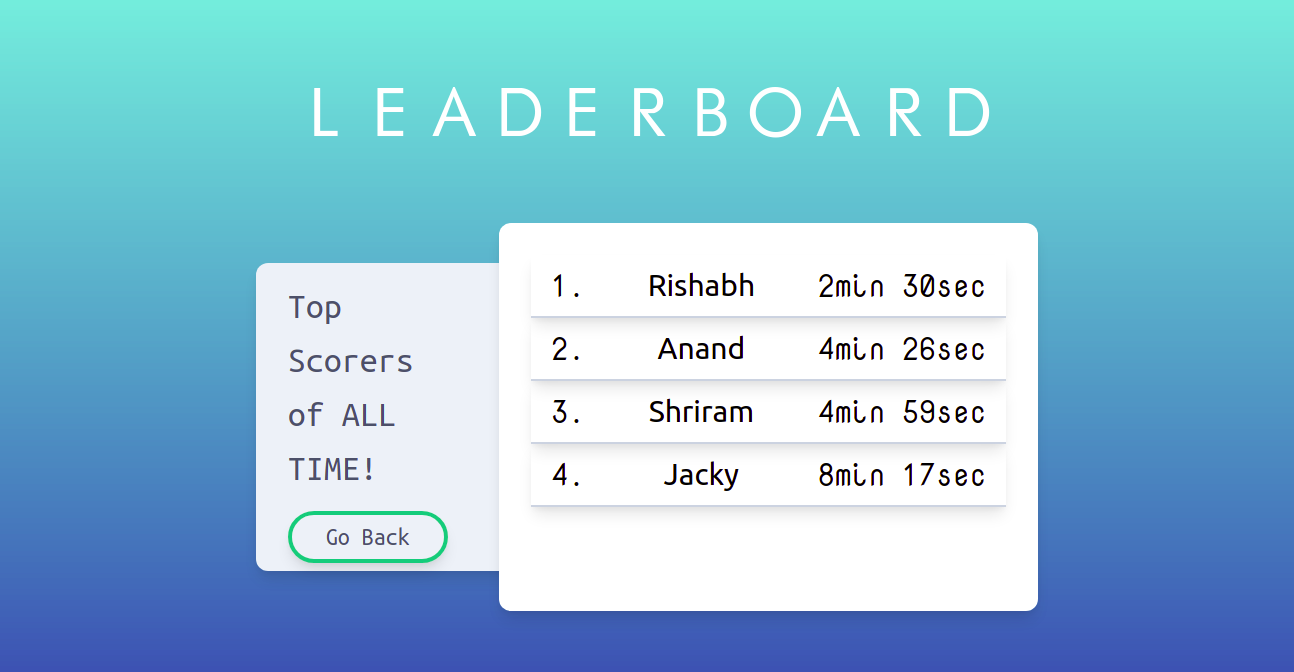
\includegraphics{leaderboard}
        \caption{Leaderboards Table}
        \label{fig:leaderboard}
    \end{figure}
    \begin{lstlisting}[language=Python, caption=mainapp/models.py]
    from django.db import models
    from typing import Union

    class GameBoards(models.Model):
        # An autoincrementing ID column which will be used as primary key is automatically added.
        game_board = models.TextField()
        check_board = models.TextField()
        def __str__(self) -> int:
            return self.id
    
    class Leaderboard(models.Model):
        name = models.CharField(max_length=20, default="Player", blank=False)
        time = models.IntegerField()
    
        def __str__(self) -> str: 
            return ", ".join([self.name, str(self.time)])
    \end{lstlisting}
    \textbf{Views and Forms}
    \begin{lstlisting}[language=Python, caption=mainapp/views.py]
from django.shortcuts import render, redirect
from django import http
from django.views.decorators.http import require_POST, require_GET
from django.db.models import Max
import json

from utils.classes import BoardsQueue
from utils.exceptions import QueueUnderflowError

from .models import GameBoards, Leaderboard
from .forms import AddToLeaderboardForm

queue = BoardsQueue()

lower, upper = 0, 11    # ID range to load to queue
# filling queue with tables saved on the database
for result in GameBoards.objects.filter(id__in=list(range(lower, upper))):
    queue.enqueue([result.id, json.loads(result.game_board), json.loads(result.check_board)])
else:
    lower, upper = 11, 21

@require_GET
def index(request):
    return render(request, "mainapp/index.html", {})

@require_GET
def game(request):
    global upper, lower
    try:
        board_id ,game_board, check_board = queue.dequeue()
    except QueueUnderflowError:
        if upper == 101:        #there are currently only 100 items on the database, so it loops back to the starting.
            lower, upper = 0, 11
        else:
            lower += 10
            upper += 10

        for result in GameBoards.objects.filter(id__in=list(range(lower, upper))):  #loading new tables from database
            queue.enqueue([result.id, json.loads(result.game_board), json.loads(result.check_board)])
        else:
            lower, upper = upper, upper + 10

        board_id, game_board, check_board = queue.dequeue()
    context = {'board_id': board_id, 'game_board': game_board, 'check_board': check_board, 'form': AddToLeaderboardForm()}
    
    return render(request, "mainapp/game.html", context)

def result(request):
    if request.method == 'POST':
        form = AddToLeaderboardForm(request.POST)
        if form.is_valid():
            time = form.cleaned_data['time']
            username = form.cleaned_data['username']

        current_worst = Leaderboard.objects.all().aggregate(Max('time'))
        if time < current_worst['time__max']:
            new = Leaderboard(name=username, time=time)
            new.save()

        return redirect('index') 

def leaderboard(request, home=""):
    if home == "lb":
        data = Leaderboard.objects.all().order_by('time')
        formatted_data = [[entry.name, entry.time] for entry in data][:10]
        context = {"data": formatted_data}.
        return render(request, "mainapp/leaderboard.html", context)
    else:
        return redirect("index")
    \end{lstlisting}
    Variables declared in the \textit{context} dictionary are passed onto the templates.\\
    \newline
    A \emph{form} was used to send the player's data over HTTP POST request, back to the server, if they have to be added to the leaderboard.
    \begin{lstlisting}[language=Python, caption=mainapp/forms.py]
from django import forms

class AddToLeaderboardForm(forms.Form):
    username = forms.CharField()
    time = forms.IntegerField()
    \end{lstlisting}
    Sudoku game boards were prepared before hand, and stored in the database. Small chunks were retrieved on demand and placed in a queue, to serve to live users.
    Functions and classes related to preparing the boards were made in the \texttt{utils} directory in the project.\\
    \begin{lstlisting}[language=Python, caption=utils/classes.py]
from random import shuffle, randint
import typing
import utils.exceptions

BoardType = typing.List[typing.List[typing.Union[None, int]]]    # type hint alias for board - a list of lists
      # with int or None as values
class Sudoku:
    """" A class that acts like a sudoku puzzle. """

    def __init__(self):  # noqa: ANN204
        self.counter = 1
        self.top_boxes = [_Box() for _ in range(3)]
        self.mid_boxes = [_Box() for _ in range(3)]
        self.bottom_boxes = [_Box() for _ in range(3)]

        self.original = [
            [1, 2, 3, 4, 5, 6, 7, 8, 9],
            [4, 5, 6, 7, 8, 9, 1, 2, 3],
            [7, 8, 9, 1, 2, 3, 4, 5, 6],
            [2, 3, 1, 5, 6, 4, 8, 9, 7],
            [5, 6, 4, 8, 9, 7, 2, 3, 1],
            [8, 9, 7, 2, 3, 1, 5, 6, 4],
            [3, 1, 2, 6, 4, 5, 9, 7, 8],
            [6, 4, 5, 9, 7, 8, 3, 1, 2],
            [9, 7, 8, 3, 1, 2, 6, 4, 5]
        ]

        self.generator()
        self.full_board = self.get_all_row_values()
        self.puzzle_maker()

    # Getter methods
    def get_column_values(self, index: int) -> list:  # returns column values in the form of
        box_index = index // 3  # a list. Indexing from 0-8 from
        element_index = index % 3  # left to right.
        column = []
        for i in range(9):
            if i % 3 == 0 and i > 1:
                box_index += 3
                element_index -= 9
            element = self[box_index][element_index]
            column.append(element.get_value())  # appends value of the element.
            element_index += 3
        return column

    def get_row_values(self, index: int) -> list:  # returns row values in the form of a list.
        box_index = (index // 3) * 3  # Indexing from 0-8 from top to bottom
        element_index = index % 3 * 3
        row = []
        for i in range(9):
            if i % 3 == 0 and i > 1:
                box_index += 1
                element_index -= 3
            element = self[box_index][element_index]
            row.append(element.get_value())
            element_index += 1
        return row

    def get_all_row_values(self) -> list:  # Return a list of all the rows.
        rows = []
        for i in range(9):
            row = self.get_row_values(i)
            rows.append(row)
        return rows

    # Puzzle-Generation methods
    def possible_cell_values(self, row: int, col: int) -> list:

        element_possibility = [1, 2, 3, 4, 5, 6, 7, 8, 9]

        for col_value in self.get_column_values(col):
            if col_value in element_possibility:  # Reoccurring in the same column
                element_possibility.remove(col_value)

        for row_value in self.get_row_values(row):
            if row_value in element_possibility:  # Reoccurring in the same row
                element_possibility.remove(row_value)

        for m in element_possibility:
            if m in [self[(row // 3) * 3 + col // 3][n].get_value() for n in range(9)]:
                element_possibility.remove(m)

        return element_possibility

    @staticmethod
    def check_complete(grid: list) -> bool:
        for i in grid:
            for x in i:
                if x == 0:
                    return False
        return True

    def generator(self) -> None:

        shuffled = []

        for i in range(3):
            rows = [self.original[i * 3], self.original[(i * 3) + 1], self.original[(i * 3) + 2]]

            shuffle(rows)
            shuffled.extend(rows)

        self.set_value_of_grid(shuffled, "row")
        shuffled = []

        for i in range(3):
            cols = [self.get_row_values(i * 3), self.get_row_values((i * 3) + 1), self.get_row_values((i * 3) + 2)]

            shuffle(cols)
            shuffled.extend(cols)

        self.set_value_of_grid(shuffled, "col")

    def set_value_of_grid(self, list_val: list, index_type: str) -> None:

        if index_type == "row":
            for box in range(9):
                for element in range(9):
                    self[box][element].set_value(list_val[(box // 3) * 3 + element // 3][(box % 3) * 3 + element % 3])
        elif index_type == "col":
            for box in range(9):
                for element in range(9):
                    self[box][element].set_value(list_val[(box % 3) * 3 + element % 3][(box // 3) * 3 + element // 3])

    def unique_sol_check(self, grid: list) -> bool:

        # Recursive method to check whether there is a unique solution for a number removed from grid
        for i in range(81):

            row = i // 9
            col = i % 9

            if grid[row][col] == 0:
                for value in range(10):
                    if value in self.possible_cell_values(row, col):
                        grid[row][col] = value
                        self.set_value_of_grid(grid, "row")
                        if self.check_complete(grid):
                            self.counter += 1
                            break
                        else:
                            if self.unique_sol_check(grid):
                                return True
                break
        grid[row][col] = 0
        self.set_value_of_grid(grid, "row")

    def puzzle_maker(self) -> None:

        # adds spaces to the finished board
        attempts = 5
        while attempts > 0:
            row = randint(0, 8)
            col = randint(0, 8)
            while self[row][col].get_value() == 0:
                row = randint(0, 8)
                col = randint(0, 8)
            backup = self[row][col].get_value()
            self[row][col].set_value(0)

            copy = self.get_all_row_values()

            self.counter = 0
            self.unique_sol_check(copy)

            if self.counter != 1:
                self[row][col].set_value(backup)
                attempts -= 1
    
    @staticmethod
    def check(user_input: list, full_board: list) -> typing.Union[bool, list]:

        if user_input == full_board:
            return True
        else:
            return [[True if full_board[row][col] == user_input[row][col] else False for col in range(9)] for row in range(9)]

    # operator overloading methods.
    def __iter__(self):  # noqa: ANN204
        for i in self.top_boxes:  # x here is a box
            yield i  # iterates through the boxes in the same way as
        for i in self.mid_boxes:  # a matrix; i.e. left to right.
            yield i
        for i in self.bottom_boxes:
            yield i

    def __getitem__(self, index: int):  # noqa: ANN204
        count = 0  # returns box object at index 3
        for i in self:
            if count == index:
                return i
            count += 1

    def __eq__(self, b: "Sudoku") -> bool:  # functionality -> sudoku1 == sudoku2
        for box in range(9):  # compares all values of both sudokus.
            for element in range(9):
                if self[box][element].get_value() != b[box][element].get_value(): return False
        return True


class _Box:
    """ A class that acts like one of the nine 3x3 boxes in sudoku. """

    def __init__(self):  # noqa: ANN204
        self.top_row = [_Element() for _ in range(3)]
        self.mid_row = [_Element() for _ in range(3)]
        self.bottom_row = [_Element() for _ in range(3)]

    # Operator overloading methods
    def __iter__(self):  # noqa: ANN204
        for element in self.top_row:  # Iterates in the same way as a matrix
            yield element  # i.e. from left to right.
        for element in self.mid_row:
            yield element
        for element in self.bottom_row:
            yield element

    def __getitem__(self, index: int):  # noqa: ANN204
        count = 0  # returns value of specified index.
        for element in self:  # indexing from 0-9; indexing is in the same way
            if count == index:  # as a matrix.
                return element
            count += 1

    def __setitem__(self, index: int, val: typing.Union[int, None]):  # noqa: ANN204
        count = 0  # assignment at a specific index.
        for element_place in range(9):
            if count == element_place:
                self[element_place].set_value(val)
            count += 1

    def __contains__(self, val: typing.Union[int, None]) -> bool:  # functionality -> val in box
        for element in self:  # returns True or False.
            if element.get_value() == val:
                return True
        return False


class _Element:
    """ A class that acts as the element(number) in one of the boxes of sudoku. """

    def __init__(self, value: typing.Optional[int]=None):   # noqa: ANN204
        self._value = value  # The value the element has.

    # getter methods.
    def get_value(self) -> typing.Any:  # To access the value this element has.
        return self._value

    # setter methods.
    def set_value(self, value: typing.Union[int, None]) -> None:  # To access the value this element will have.
        self._value = value


class BoardsQueue:
    """FIFO queue containing upto {max_length} Sudoku boards at a time.
    Front of the queue is the index 0, and the back is -1.
    
    Raises: QueueOverflowError -> on trying to insert into the queue beyond it's specified max_size
            QueueUnderflowError -> on trying to get an item from the empty queue."""
    def __init__(self, max_size: int=10):   # noqa: ANN204
        self._queue = []
        self.max_size = max_size

    def enqueue(self, board: list) -> None:
        if len(self._queue) > self.max_size:
            raise utils.exceptions.QueueOverflowError
        
        self._queue.append(board)

    def dequeue(self) -> typing.Union[list, None]:
        if len(self._queue) == 0:
            raise utils.exceptions.QueueUnderflowError
        
        return self._queue.pop(0)
    \end{lstlisting}
    Some exceptions that are raised by the queue are defined in \texttt{utils/exceptions.py} file. These exceptions inherit from the base \code{Exception} class.
    \newline
    % add utils code here, for sudoku and queue
    \textbf{URLconf}\\
    URL configuration, or \textit{URLconf}, is the process of defining URLs for your app. This is done by writing some Python code, which acts as a mapping between URL path expressions, and their corresponding view functions.
    The URLconf for this project has two layers:
    \begin{enumerate}
        \item \textit{Project-level URLs}\\
        \begin{lstlisting}[language=Python, caption=sudoku/urls.py]
from django.contrib import admin
from django.urls import path, include

urlpatterns = [
    path('admin/', admin.site.urls),
    path('', include('mainapp.urls')),
]
        \end{lstlisting}
        This simply redirects every URL except \texttt{/admin} to the URL configuration for \texttt{mainapp}.
        \item \textit{App-level URLs}
        \begin{lstlisting}[language=Python, caption=mainapp/urls.py]
from django.urls import path
from . import views

urlpatterns = [
    path("", views.index, name="index"),
    path("game", views.game, name="game"),
    path("result", views.result, name="result"),
    path("leaderboard/<home>", views.leaderboard, name="leaderboard")
]
        \end{lstlisting}
        This maps a URL to a specific view function defined in \texttt{views.py}; when any of these URLs are reached, their corresponding view function is automatically called.
    \end{enumerate}
    
        \subsection{Frontend}
    Frontend, also referred to as the \emph{"client-side"}, is the part of the website that you can see and interact with directly.\\
    
    Web pages are designed using three languages:
    \begin{itemize}
        \item Hypertext Markup Language (HTML)\\
        It is used for laying out the structure of the webpage 
        and for making forms that share data with the backend.
        \item Cascading Style Sheets (CSS)\\
        It is used to improve the page visually.
        \item JavaScript\\
        It is a programming language that can be used in both frontend and backend. It adds behaviour to web pages and
        makes them interactive. 
    \end{itemize}
    
    As CSS alone is time consuming to write, frameworks are used to speed up the development.
    In our project TailwindCSS framework has been used.
    
    \newpage
    \subsection{Output}
    
    \begin{figure}[h!]
        
\includegraphics[scale=0.34]{index-webpage}
        \caption{Index Page}
        \label{fig:index-webpage}
    \end{figure}
    
    \begin{figure}[h!]
        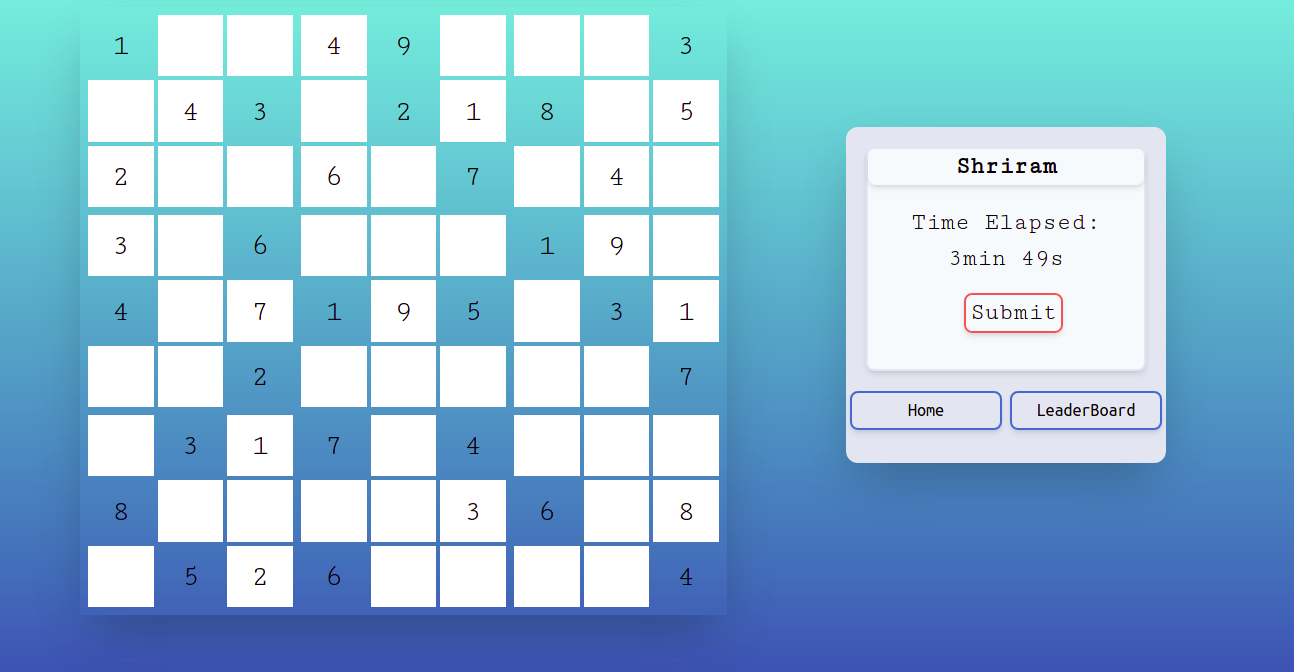
\includegraphics[scale=0.35]{game-webpage}
        \caption{Game Page}
        \label{fig:game-webpage}
    \end{figure}
    
    \begin{figure}[h!]
        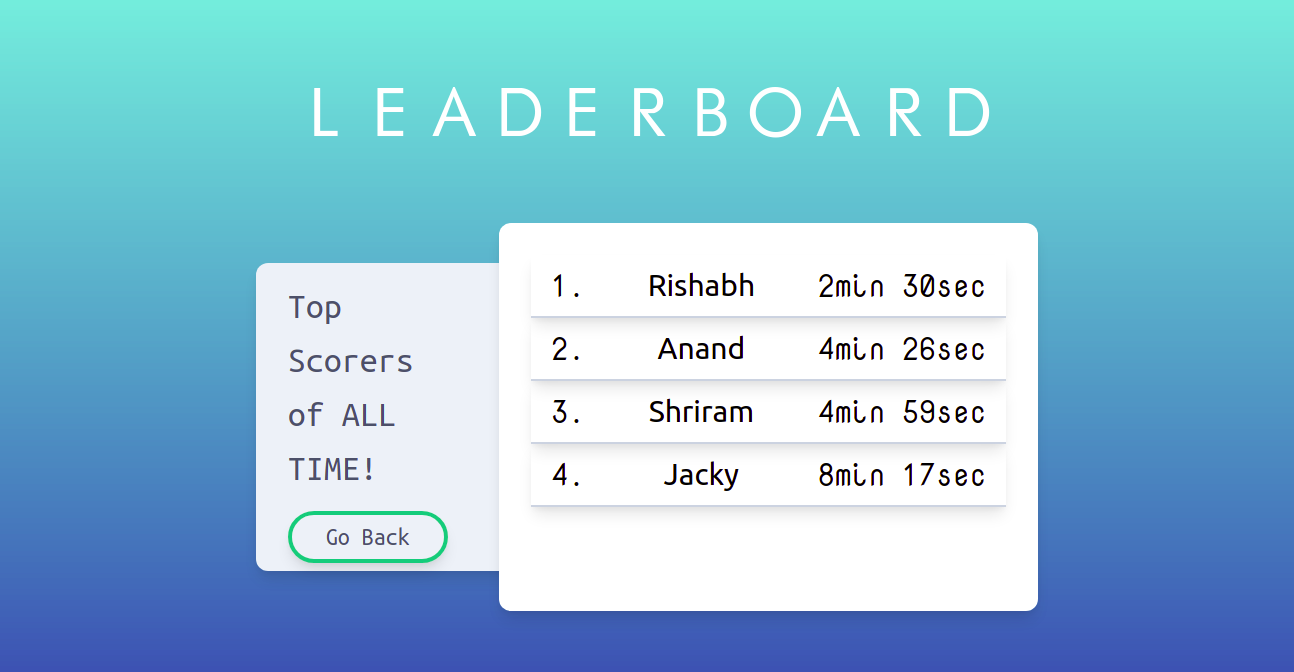
\includegraphics[scale=0.35]{leaderboard-webpage}
        \caption{Leaderboard Page}
        \label{fig:leaderboard-webpage}
    \end{figure}
    
  \newpage
  \addcontentsline{toc}{section}{References}
  \begin{thebibliography}{8}
  \bibitem{python}
  Python 3. \textit{Interpreted, high-level, general-purpose programming language.}
  \\\texttt{https://docs.python.org/3/}
  
  \bibitem{django}
  Django. \textit{The Web Framework for perfectionists with a deadline}
  \\\texttt{https://docs.djangoproject.com/en/3.1/}
  
  \bibitem{tailwind}
  TailwindCSS. \textit{A utility-first CSS framework packed with classes.}
  \\\texttt{https://tailwindcss.com/docs}
  
  \bibitem{mysql}
  MySQL Database. \textit{Fast relational database.}
  \\\texttt{https://dev.mysql.com/doc/}
  
  \bibitem{wikipedia}
  Wikipedia. \textit{The free online encyclopedia.}
  \\\texttt{https://www.wikipedia.com}
  
  \bibitem{stackoverflow}
  Stackoverflow. \textit{Where developers learn, share and build.}
  \\\texttt{https://stackoverflow.com/}
  
  \bibitem{latex}
  \LaTeX. \textit{High quality type-setting system.}
  \\\texttt{https://www.latex-project.org/help/documentation/}
  
  \bibitem{git}
  Git SCM \textit{Distributed Version-Control System.}
  \\\texttt{https://git-scm.com/}
  
  \end{thebibliography}
  
  
\end{document}
